\documentclass{book}
\usepackage[a4paper,top=2.5cm,bottom=2.5cm,left=2.5cm,right=2.5cm]{geometry}
\usepackage{makeidx}
\usepackage{natbib}
\usepackage{graphicx}
\usepackage{multicol}
\usepackage{float}
\usepackage{listings}
\usepackage{color}
\usepackage{ifthen}
\usepackage[table]{xcolor}
\usepackage{textcomp}
\usepackage{alltt}
\usepackage{ifpdf}
\ifpdf
\usepackage[pdftex,
            pagebackref=true,
            colorlinks=true,
            linkcolor=blue,
            unicode
           ]{hyperref}
\else
\usepackage[ps2pdf,
            pagebackref=true,
            colorlinks=true,
            linkcolor=blue,
            unicode
           ]{hyperref}
\usepackage{pspicture}
\fi
\usepackage[utf8]{inputenc}
\usepackage{mathptmx}
\usepackage[scaled=.90]{helvet}
\usepackage{courier}
\usepackage{sectsty}
\usepackage{amssymb}
\usepackage[titles]{tocloft}
\usepackage{doxygen}
\lstset{language=C++,inputencoding=utf8,basicstyle=\footnotesize,breaklines=true,breakatwhitespace=true,tabsize=8,numbers=left }
\makeindex
\setcounter{tocdepth}{3}
\renewcommand{\footrulewidth}{0.4pt}
\renewcommand{\familydefault}{\sfdefault}
\hfuzz=15pt
\setlength{\emergencystretch}{15pt}
\hbadness=750
\tolerance=750
\begin{document}
\hypersetup{pageanchor=false,citecolor=blue}
\begin{titlepage}
\vspace*{7cm}
\begin{center}
{\Large My Project }\\
\vspace*{1cm}
{\large Generated by Doxygen 1.8.1.2}\\
\vspace*{0.5cm}
{\small Fri Oct 24 2014 11:39:54}\\
\end{center}
\end{titlepage}
\clearemptydoublepage
\pagenumbering{roman}
\tableofcontents
\clearemptydoublepage
\pagenumbering{arabic}
\hypersetup{pageanchor=true,citecolor=blue}
\chapter{Liste des types de multimedia\-:}
\label{md_README}
\hypertarget{md_README}{}

\begin{DoxyItemize}
\item Base( nom\+:string, date\+\_\+de\+\_\+creation\+:time\+\_\+t, path\+:string )
\item \hyperlink{classPhoto}{Photo( \mbox{[} ceux de Base \mbox{]}, lieu\+:string )}
\item \hyperlink{classVideo}{Video( \mbox{[} ceux de Base \mbox{]}, duree\+:int )}
\item \hyperlink{classFilm}{Film( \mbox{[} ceux de Video \mbox{]}, nombre\+\_\+de\+\_\+chaiptres\+:int, duree\+\_\+des\+\_\+chaiptres\+:int\mbox{[}$\,$\mbox{]} )}
\end{DoxyItemize}

\section*{7e étape }

Ceux qui ont besoin de leurs propres destructeurs sont ceux avec des pointeurs comme variables. Ca veut dire aussi des tableaux, donc \hyperlink{classFilm}{Film}.

Il faut aussi ecrire un constructeur de copie pour \hyperlink{classFilm}{Film}, pour copier profondement le tableau. 
\chapter{Class Index}
\section{Class Hierarchy}
This inheritance list is sorted roughly, but not completely, alphabetically\-:\begin{DoxyCompactList}
\item \contentsline{section}{Base\-Object}{\pageref{classBaseObject}}{}
\begin{DoxyCompactList}
\item \contentsline{section}{Photo}{\pageref{classPhoto}}{}
\item \contentsline{section}{Video}{\pageref{classVideo}}{}
\begin{DoxyCompactList}
\item \contentsline{section}{Film}{\pageref{classFilm}}{}
\end{DoxyCompactList}
\end{DoxyCompactList}
\end{DoxyCompactList}

\chapter{Class Index}
\section{Class List}
Here are the classes, structs, unions and interfaces with brief descriptions\-:\begin{DoxyCompactList}
\item\contentsline{section}{\hyperlink{classBaseObject}{Base\-Object} \\*Base multimedia-\/type file object }{\pageref{classBaseObject}}{}
\item\contentsline{section}{\hyperlink{classPhoto}{Photo} \\*\hyperlink{classPhoto}{Photo} file object }{\pageref{classPhoto}}{}
\item\contentsline{section}{\hyperlink{classVideo}{Video} \\*\hyperlink{classVideo}{Video} file object }{\pageref{classVideo}}{}
\end{DoxyCompactList}

\chapter{Class Documentation}
\hypertarget{classBaseObject}{\section{Base\-Object Class Reference}
\label{classBaseObject}\index{Base\-Object@{Base\-Object}}
}


Base multimedia-\/type file object.  




{\ttfamily \#include $<$Base\-Object.\-h$>$}

Inheritance diagram for Base\-Object\-:\begin{figure}[H]
\begin{center}
\leavevmode
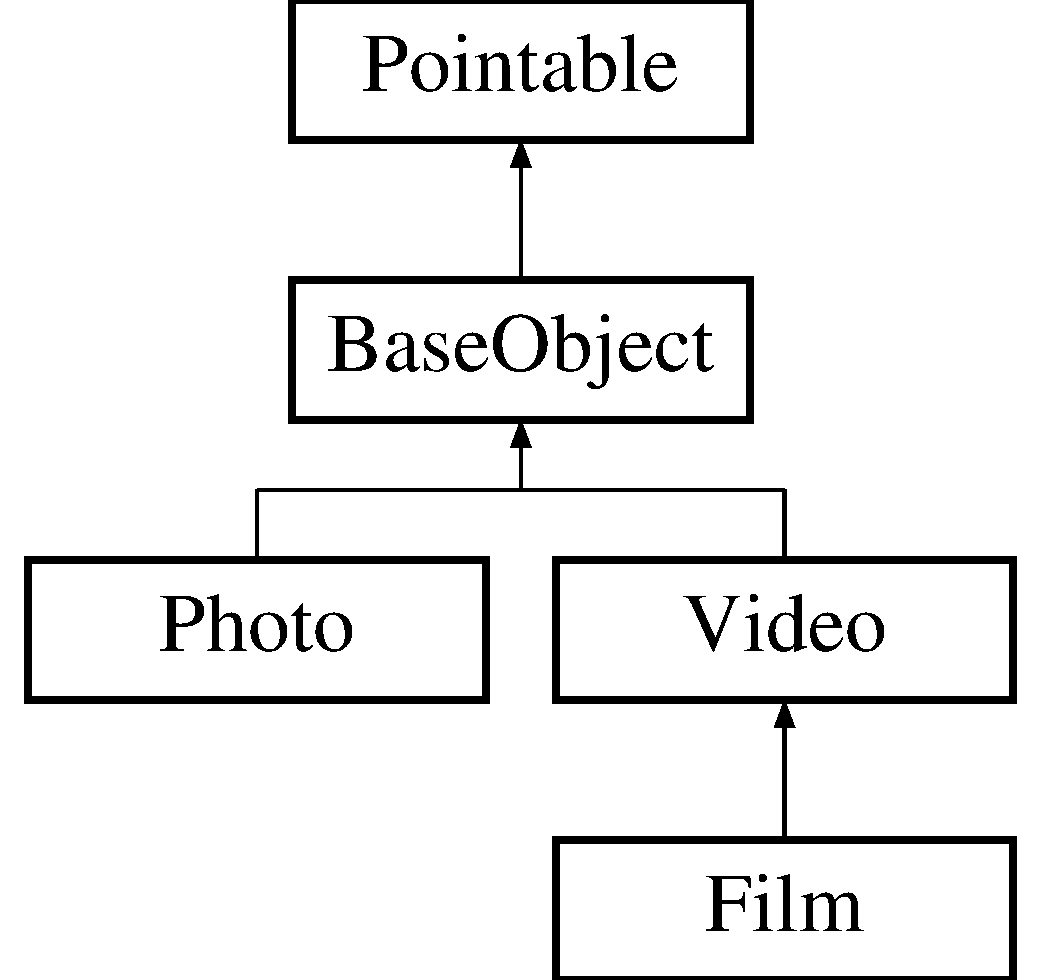
\includegraphics[height=3.000000cm]{classBaseObject}
\end{center}
\end{figure}
\subsection*{Public Member Functions}
\begin{DoxyCompactItemize}
\item 
\hypertarget{classBaseObject_ac9e64a371856dc974183c1b04bfdd0c9}{\hyperlink{classBaseObject_ac9e64a371856dc974183c1b04bfdd0c9}{Base\-Object} ()}\label{classBaseObject_ac9e64a371856dc974183c1b04bfdd0c9}

\begin{DoxyCompactList}\small\item\em Parameterless Constructor. \end{DoxyCompactList}\item 
\hypertarget{classBaseObject_aef7d506580d526367abe614c614aaf43}{\hyperlink{classBaseObject_aef7d506580d526367abe614c614aaf43}{Base\-Object} (std\-::string, time\-\_\-t, std\-::string)}\label{classBaseObject_aef7d506580d526367abe614c614aaf43}

\begin{DoxyCompactList}\small\item\em Parametered Constructor. \end{DoxyCompactList}\item 
virtual \hyperlink{classBaseObject_a83eecfd3bdaffda4e6c7d0fb98747f96}{$\sim$\-Base\-Object} ()
\begin{DoxyCompactList}\small\item\em Parameterless Destructor. \end{DoxyCompactList}\item 
\hypertarget{classBaseObject_a813ed6b0e98919c44c5ddf95495bfa2d}{std\-::string \hyperlink{classBaseObject_a813ed6b0e98919c44c5ddf95495bfa2d}{get\-Name} () const }\label{classBaseObject_a813ed6b0e98919c44c5ddf95495bfa2d}

\begin{DoxyCompactList}\small\item\em Returns name of multimedia object (track name, movie title etc) \end{DoxyCompactList}\item 
\hypertarget{classBaseObject_a1d9abdd27cea258333a27d505c57e857}{time\-\_\-t \hyperlink{classBaseObject_a1d9abdd27cea258333a27d505c57e857}{get\-Creation\-Date} () const }\label{classBaseObject_a1d9abdd27cea258333a27d505c57e857}

\begin{DoxyCompactList}\small\item\em Returns date of creation as time\-\_\-t. \end{DoxyCompactList}\item 
\hypertarget{classBaseObject_a46ce6977e2a06f0785aca14454df9d94}{std\-::string \hyperlink{classBaseObject_a46ce6977e2a06f0785aca14454df9d94}{get\-Path} () const }\label{classBaseObject_a46ce6977e2a06f0785aca14454df9d94}

\begin{DoxyCompactList}\small\item\em Returns unix path (including filename) of object. \end{DoxyCompactList}\item 
\hypertarget{classBaseObject_a3999488d0dd4e825641ece8f332385e1}{void \hyperlink{classBaseObject_a3999488d0dd4e825641ece8f332385e1}{set\-Name} (std\-::string)}\label{classBaseObject_a3999488d0dd4e825641ece8f332385e1}

\begin{DoxyCompactList}\small\item\em Sets name of multimedia object (track name, movie title etc) \end{DoxyCompactList}\item 
\hypertarget{classBaseObject_aeeb327051d61bd727722f583fa0bc41c}{void \hyperlink{classBaseObject_aeeb327051d61bd727722f583fa0bc41c}{set\-Creation\-Date} (time\-\_\-t)}\label{classBaseObject_aeeb327051d61bd727722f583fa0bc41c}

\begin{DoxyCompactList}\small\item\em Sets date of creation as time\-\_\-t. \end{DoxyCompactList}\item 
\hypertarget{classBaseObject_a06461859fe33fc77fee0b74dbbe1b57d}{void \hyperlink{classBaseObject_a06461859fe33fc77fee0b74dbbe1b57d}{set\-Path} (std\-::string)}\label{classBaseObject_a06461859fe33fc77fee0b74dbbe1b57d}

\begin{DoxyCompactList}\small\item\em Sets unix path (including filename) of object. \end{DoxyCompactList}\item 
\hypertarget{classBaseObject_aab08eee6684fdfa0852b1f914379b9c4}{virtual std\-::string \hyperlink{classBaseObject_aab08eee6684fdfa0852b1f914379b9c4}{to\-String} () const }\label{classBaseObject_aab08eee6684fdfa0852b1f914379b9c4}

\begin{DoxyCompactList}\small\item\em Returns multi-\/line string containing formatted description of object. \end{DoxyCompactList}\item 
void \hyperlink{classBaseObject_a9bad65dddde7dec1ea622edce664cc9f}{print} () const 
\begin{DoxyCompactList}\small\item\em Prints formatted description of object. \end{DoxyCompactList}\end{DoxyCompactItemize}


\subsection{Detailed Description}
Base multimedia-\/type file object. 

This class is the base class for all objects which describe multimedia files in the project. 

\subsection{Constructor \& Destructor Documentation}
\hypertarget{classBaseObject_a83eecfd3bdaffda4e6c7d0fb98747f96}{\index{Base\-Object@{Base\-Object}!$\sim$\-Base\-Object@{$\sim$\-Base\-Object}}
\index{$\sim$\-Base\-Object@{$\sim$\-Base\-Object}!BaseObject@{Base\-Object}}
\subsubsection[{$\sim$\-Base\-Object}]{\setlength{\rightskip}{0pt plus 5cm}Base\-Object\-::$\sim$\-Base\-Object (
\begin{DoxyParamCaption}
{}
\end{DoxyParamCaption}
)\hspace{0.3cm}{\ttfamily [virtual]}}}\label{classBaseObject_a83eecfd3bdaffda4e6c7d0fb98747f96}


Parameterless Destructor. 

Implemetation is empty as there is nothing to delete. 

\subsection{Member Function Documentation}
\hypertarget{classBaseObject_a9bad65dddde7dec1ea622edce664cc9f}{\index{Base\-Object@{Base\-Object}!print@{print}}
\index{print@{print}!BaseObject@{Base\-Object}}
\subsubsection[{print}]{\setlength{\rightskip}{0pt plus 5cm}void Base\-Object\-::print (
\begin{DoxyParamCaption}
{}
\end{DoxyParamCaption}
) const}}\label{classBaseObject_a9bad65dddde7dec1ea622edce664cc9f}


Prints formatted description of object. 

This function prints out a description of the object, usually by displaying the values of each member variable. It does this by calling the \hyperlink{classBaseObject_aab08eee6684fdfa0852b1f914379b9c4}{to\-String()} function of the object. Thus that function is virtual, so that subclasses of \hyperlink{classBaseObject}{Base\-Object} can effectively reimplement this function to include extra member data. 

The documentation for this class was generated from the following files\-:\begin{DoxyCompactItemize}
\item 
Base\-Object.\-h\item 
Base\-Object.\-cpp\end{DoxyCompactItemize}

\hypertarget{classFilm}{\section{Film Class Reference}
\label{classFilm}\index{Film@{Film}}
}


\hyperlink{classFilm}{Film} file object.  




{\ttfamily \#include $<$Film.\-h$>$}

Inheritance diagram for Film\-:\begin{figure}[H]
\begin{center}
\leavevmode
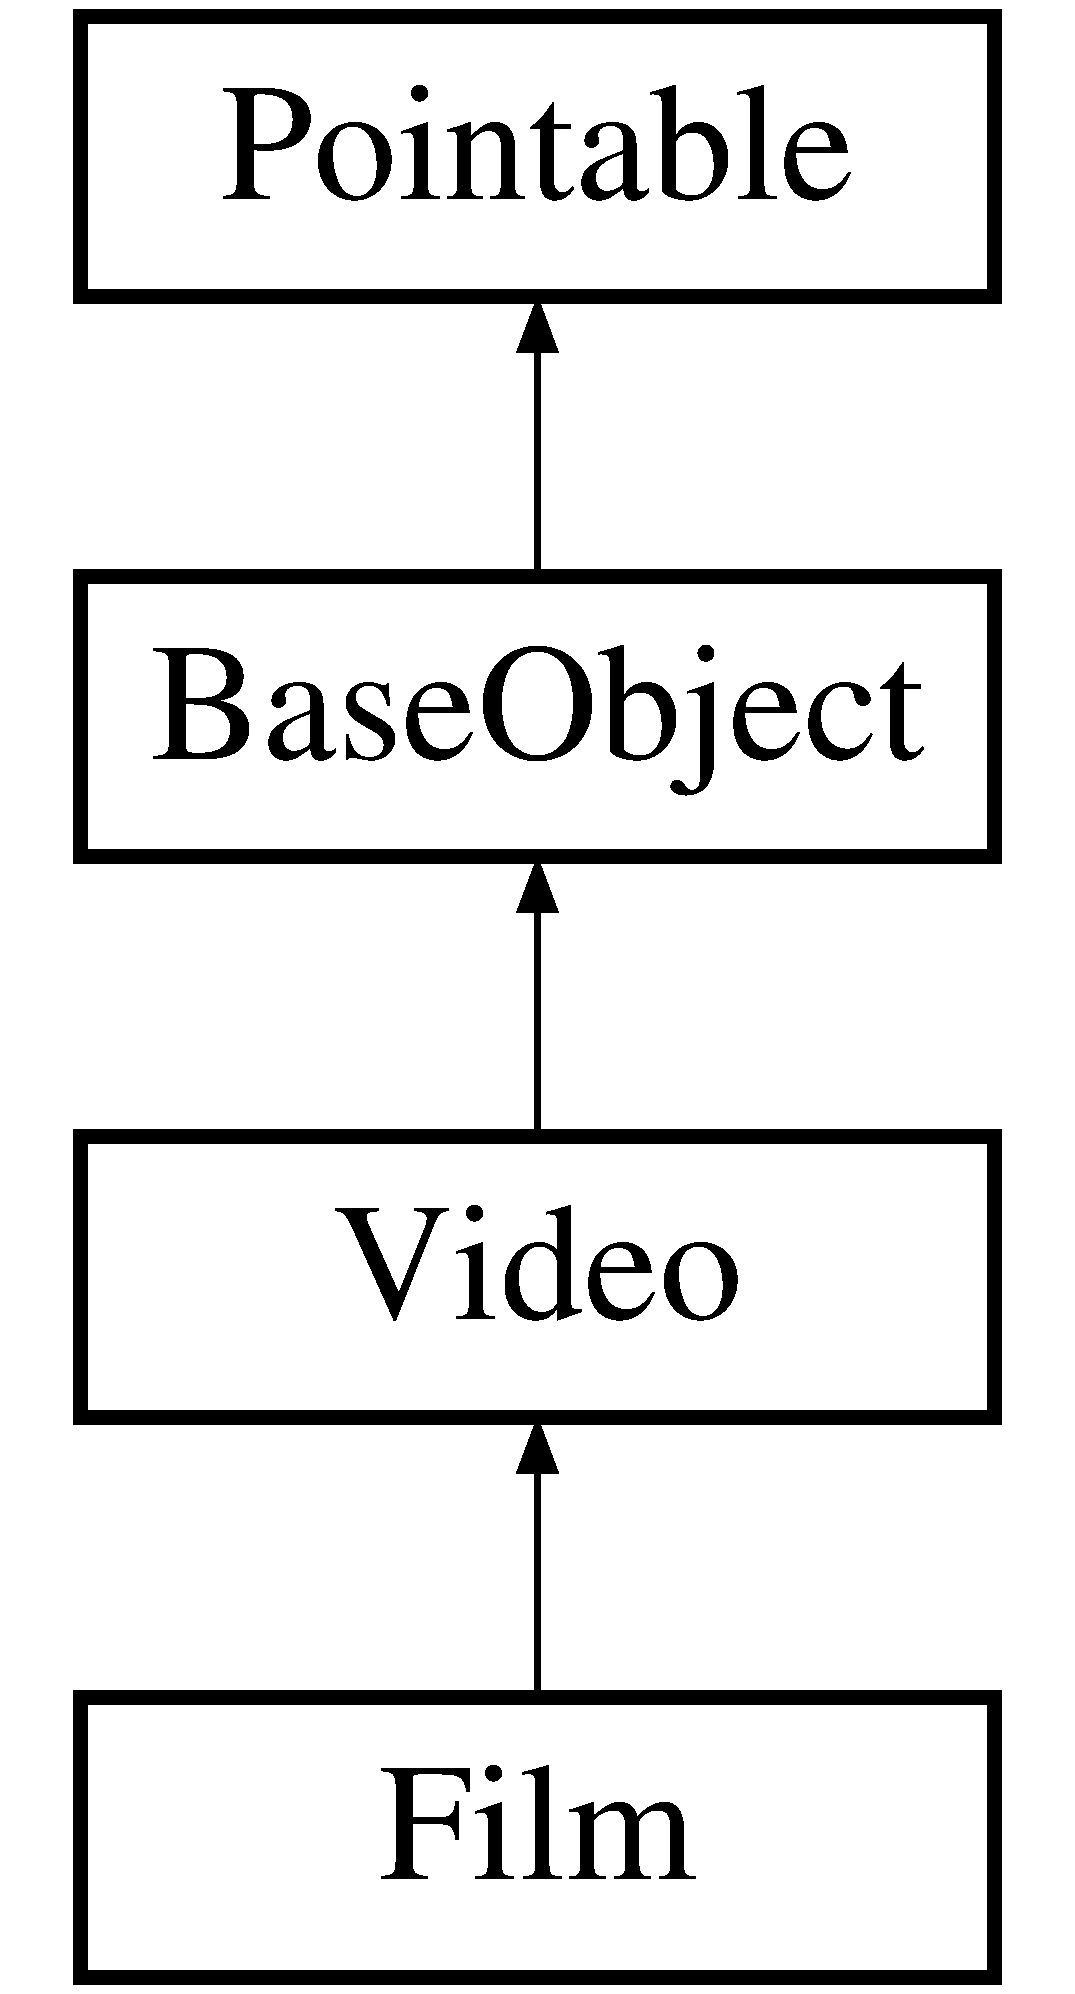
\includegraphics[height=4.000000cm]{classFilm}
\end{center}
\end{figure}
\subsection*{Public Member Functions}
\begin{DoxyCompactItemize}
\item 
\hypertarget{classFilm_a704092a2bb7629c5bf053c8011e148ee}{\hyperlink{classFilm_a704092a2bb7629c5bf053c8011e148ee}{Film} (const std\-::string \&name=\char`\"{}new film\char`\"{}, time\-\_\-t creat=time(N\-U\-L\-L), const std\-::string \&path=\char`\"{}$\sim$/new\-\_\-film\char`\"{}, int duration=0, int chapter\-\_\-count=0, int $\ast$chapters=N\-U\-L\-L)}\label{classFilm_a704092a2bb7629c5bf053c8011e148ee}

\begin{DoxyCompactList}\small\item\em Parametered Constructor. \end{DoxyCompactList}\item 
\hypertarget{classFilm_a34c9de2efb9554ce1192e4110d98806b}{\hyperlink{classFilm_a34c9de2efb9554ce1192e4110d98806b}{Film} (const \hyperlink{classFilm}{Film} \&)}\label{classFilm_a34c9de2efb9554ce1192e4110d98806b}

\begin{DoxyCompactList}\small\item\em Copy Constructor. \end{DoxyCompactList}\item 
virtual \hyperlink{classFilm_a8dab653f8a6c0635ca5ddbe0bbdd9a25}{$\sim$\-Film} ()
\begin{DoxyCompactList}\small\item\em Parameterless Destructor. \end{DoxyCompactList}\item 
\hypertarget{classFilm_a413b52608cd8103e74d3ee7ea8026e17}{virtual std\-::string \hyperlink{classFilm_a413b52608cd8103e74d3ee7ea8026e17}{to\-String} (bool=false) const }\label{classFilm_a413b52608cd8103e74d3ee7ea8026e17}

\begin{DoxyCompactList}\small\item\em Returns multi-\/line string containing formatted description of object. \end{DoxyCompactList}\item 
\hypertarget{classFilm_ab0c2831b76a6b932dfc4a6facc38870c}{void \hyperlink{classFilm_ab0c2831b76a6b932dfc4a6facc38870c}{set\-Chapters} (const int $\ast$, int)}\label{classFilm_ab0c2831b76a6b932dfc4a6facc38870c}

\begin{DoxyCompactList}\small\item\em setter for chapters array. must also pass length of array, which sets Chapter\-Count \end{DoxyCompactList}\item 
\hypertarget{classFilm_ad0fa928009af1be1c176d06d55c14e11}{const int $\ast$ \hyperlink{classFilm_ad0fa928009af1be1c176d06d55c14e11}{get\-Chapters} (void) const }\label{classFilm_ad0fa928009af1be1c176d06d55c14e11}

\begin{DoxyCompactList}\small\item\em getter for chapter array \end{DoxyCompactList}\item 
\hypertarget{classFilm_a3e07b723255ff357d3f459b08c5fa39e}{int \hyperlink{classFilm_a3e07b723255ff357d3f459b08c5fa39e}{get\-Chapter\-Count} (void) const }\label{classFilm_a3e07b723255ff357d3f459b08c5fa39e}

\begin{DoxyCompactList}\small\item\em getter for number of chapters \end{DoxyCompactList}\end{DoxyCompactItemize}


\subsection{Detailed Description}
\hyperlink{classFilm}{Film} file object. 

This class describes a \hyperlink{classFilm}{Film} object 

\subsection{Constructor \& Destructor Documentation}
\hypertarget{classFilm_a8dab653f8a6c0635ca5ddbe0bbdd9a25}{\index{Film@{Film}!$\sim$\-Film@{$\sim$\-Film}}
\index{$\sim$\-Film@{$\sim$\-Film}!Film@{Film}}
\subsubsection[{$\sim$\-Film}]{\setlength{\rightskip}{0pt plus 5cm}Film\-::$\sim$\-Film (
\begin{DoxyParamCaption}
{}
\end{DoxyParamCaption}
)\hspace{0.3cm}{\ttfamily [virtual]}}}\label{classFilm_a8dab653f8a6c0635ca5ddbe0bbdd9a25}


Parameterless Destructor. 

Deletes table of chapters. 

The documentation for this class was generated from the following files\-:\begin{DoxyCompactItemize}
\item 
Film.\-h\item 
Film.\-cpp\end{DoxyCompactItemize}

\hypertarget{classPhoto}{\section{Photo Class Reference}
\label{classPhoto}\index{Photo@{Photo}}
}


\hyperlink{classPhoto}{Photo} file object.  




{\ttfamily \#include $<$Photo.\+h$>$}

Inheritance diagram for Photo\+:\begin{figure}[H]
\begin{center}
\leavevmode
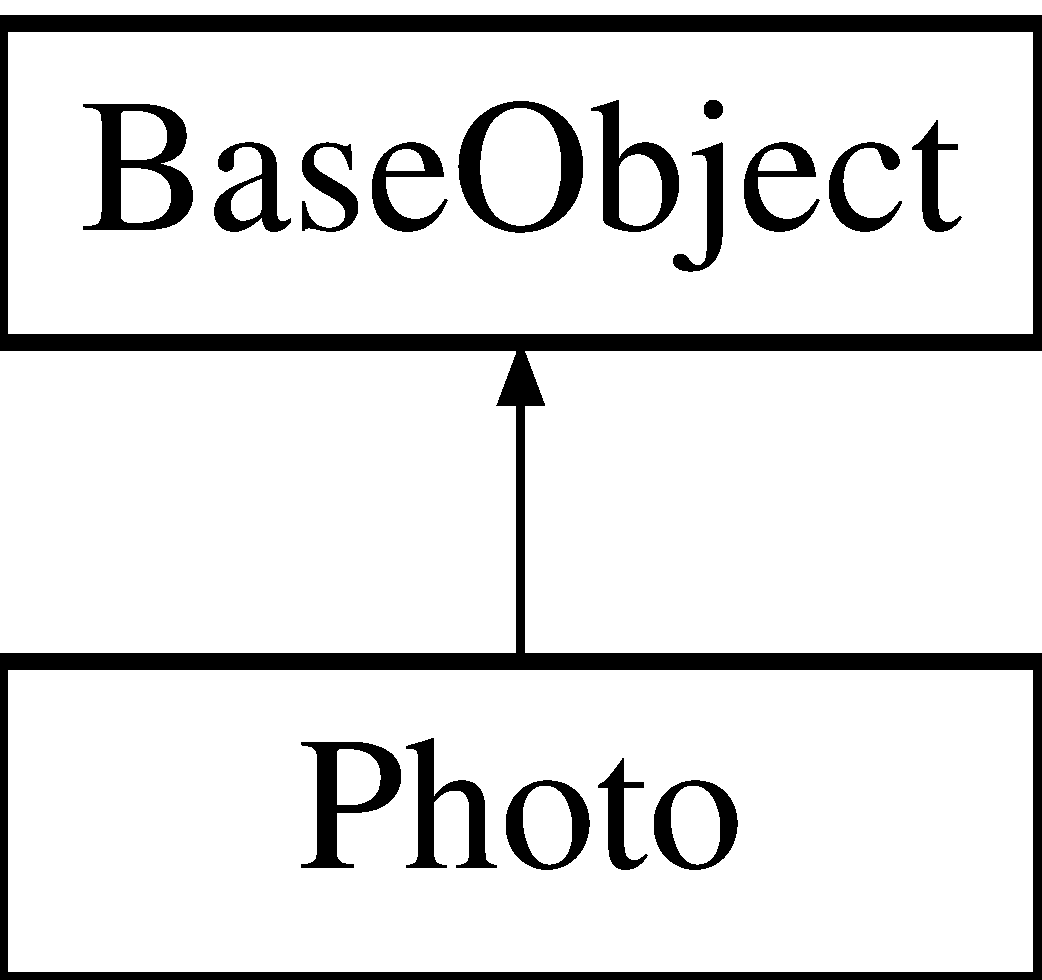
\includegraphics[height=3.000000cm]{classPhoto}
\end{center}
\end{figure}
\subsection*{Public Member Functions}
\begin{DoxyCompactItemize}
\item 
\hypertarget{classPhoto_ab07e00487a31f231f4730b3859664da5}{\hyperlink{classPhoto_ab07e00487a31f231f4730b3859664da5}{Photo} (const std\+::string \&name=\char`\"{}new photo\char`\"{}, time\+\_\+t creat=time(N\+U\+L\+L), const std\+::string \&path=\char`\"{}$\sim$/new\+\_\+photo\char`\"{}, const std\+::string \&place=\char`\"{}\char`\"{})}\label{classPhoto_ab07e00487a31f231f4730b3859664da5}

\begin{DoxyCompactList}\small\item\em Parametered Constructor. \end{DoxyCompactList}\item 
virtual \hyperlink{classPhoto_adc366234be6226600360c7cbba8e7fcf}{$\sim$\+Photo} ()
\begin{DoxyCompactList}\small\item\em Parameterless Destructor. \end{DoxyCompactList}\item 
\hypertarget{classPhoto_a8be4be2bb68b6db13ec45ff3bed71481}{virtual std\+::string \hyperlink{classPhoto_a8be4be2bb68b6db13ec45ff3bed71481}{to\+String} (void) const }\label{classPhoto_a8be4be2bb68b6db13ec45ff3bed71481}

\begin{DoxyCompactList}\small\item\em Returns multi-\/line string containing formatted description of object. \end{DoxyCompactList}\item 
\hypertarget{classPhoto_a145e0540284cbc678ef5bdb02a8fcaa8}{virtual void \hyperlink{classPhoto_a145e0540284cbc678ef5bdb02a8fcaa8}{play} ()}\label{classPhoto_a145e0540284cbc678ef5bdb02a8fcaa8}

\begin{DoxyCompactList}\small\item\em Opens file in external player. \end{DoxyCompactList}\item 
\hypertarget{classPhoto_a310123a0d107ab078bc83a80b484e2c1}{const std\+::string \& \hyperlink{classPhoto_a310123a0d107ab078bc83a80b484e2c1}{get\+Place} (void) const }\label{classPhoto_a310123a0d107ab078bc83a80b484e2c1}

\begin{DoxyCompactList}\small\item\em getter for place \end{DoxyCompactList}\item 
\hypertarget{classPhoto_ae835a7d23db2b2f6b90d1efaaf034959}{void \hyperlink{classPhoto_ae835a7d23db2b2f6b90d1efaaf034959}{set\+Place} (const std\+::string \&)}\label{classPhoto_ae835a7d23db2b2f6b90d1efaaf034959}

\begin{DoxyCompactList}\small\item\em setter for place \end{DoxyCompactList}\end{DoxyCompactItemize}


\subsection{Detailed Description}
\hyperlink{classPhoto}{Photo} file object. 

This class describes a \hyperlink{classPhoto}{Photo} object 

\subsection{Constructor \& Destructor Documentation}
\hypertarget{classPhoto_adc366234be6226600360c7cbba8e7fcf}{\index{Photo@{Photo}!````~Photo@{$\sim$\+Photo}}
\index{````~Photo@{$\sim$\+Photo}!Photo@{Photo}}
\subsubsection[{$\sim$\+Photo}]{\setlength{\rightskip}{0pt plus 5cm}Photo\+::$\sim$\+Photo (
\begin{DoxyParamCaption}
{}
\end{DoxyParamCaption}
)\hspace{0.3cm}{\ttfamily [virtual]}}}\label{classPhoto_adc366234be6226600360c7cbba8e7fcf}


Parameterless Destructor. 

Implemetation is empty as there is nothing to delete. 

The documentation for this class was generated from the following files\+:\begin{DoxyCompactItemize}
\item 
Photo.\+h\item 
Photo.\+cpp\end{DoxyCompactItemize}

\hypertarget{classVideo}{\section{Video Class Reference}
\label{classVideo}\index{Video@{Video}}
}


\hyperlink{classVideo}{Video} file object.  




{\ttfamily \#include $<$Video.\-h$>$}

Inheritance diagram for Video\-:\begin{figure}[H]
\begin{center}
\leavevmode
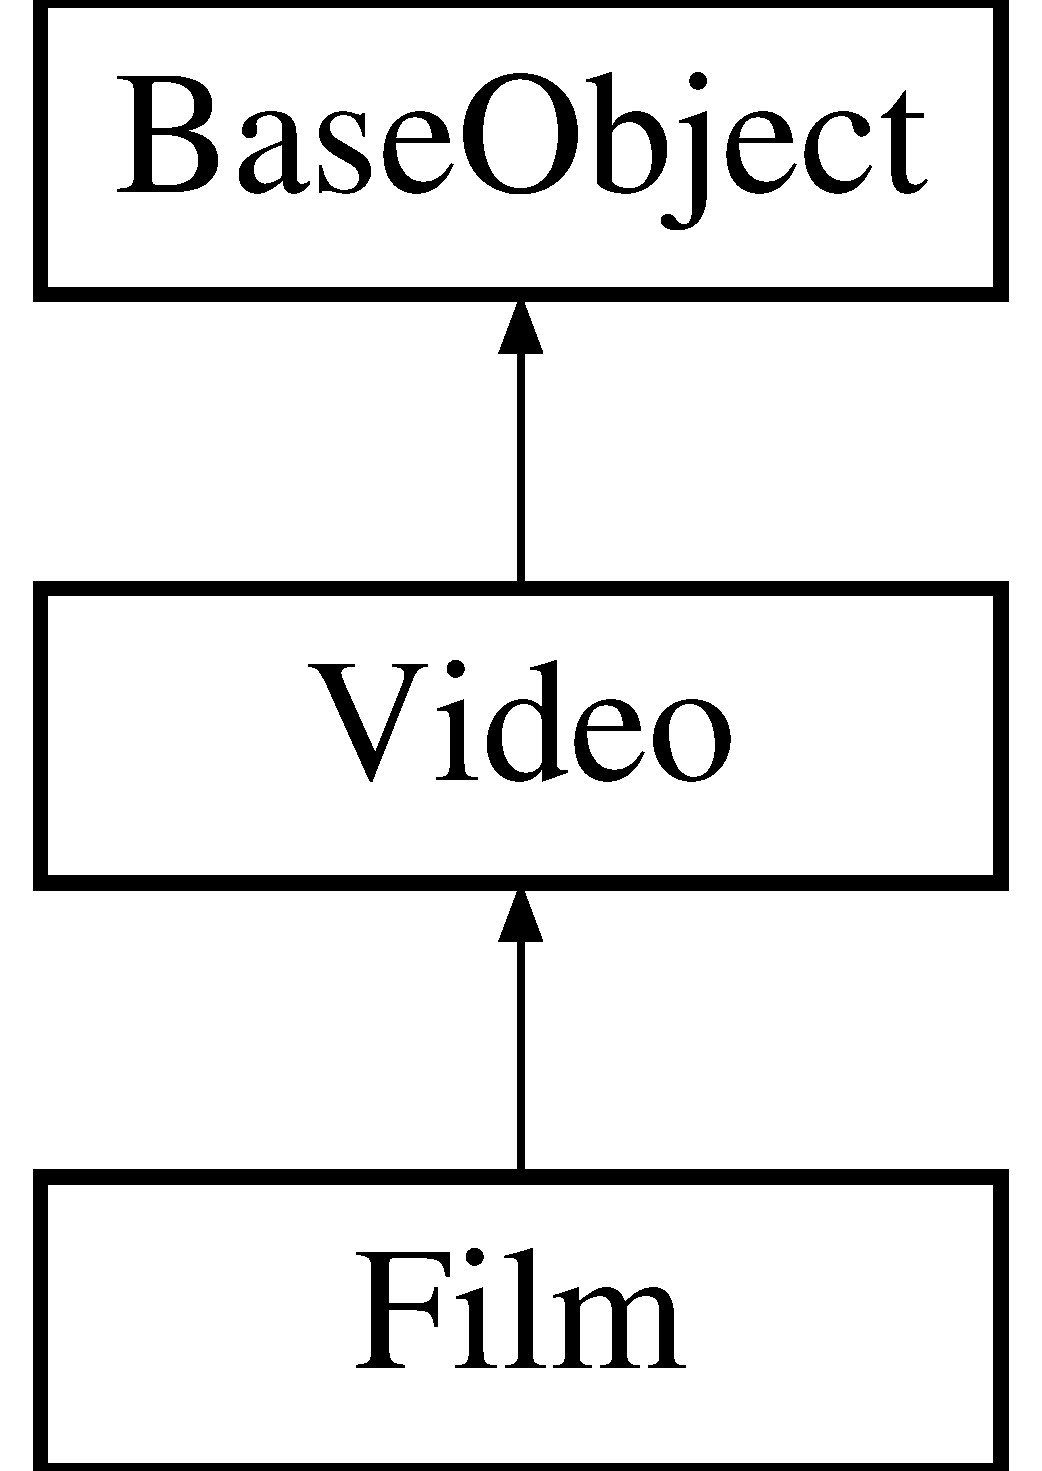
\includegraphics[height=2.000000cm]{classVideo}
\end{center}
\end{figure}
\subsection*{Public Member Functions}
\begin{DoxyCompactItemize}
\item 
\hypertarget{classVideo_ad0277d8e5772008e22ac2948e03e103b}{\hyperlink{classVideo_ad0277d8e5772008e22ac2948e03e103b}{Video} (std\-::string name=\char`\"{}new video\char`\"{}, time\-\_\-t creat=time(N\-U\-L\-L), std\-::string path=\char`\"{}$\sim$/new\-\_\-video\char`\"{}, int duration=0)}\label{classVideo_ad0277d8e5772008e22ac2948e03e103b}

\begin{DoxyCompactList}\small\item\em Parametered Constructor. \end{DoxyCompactList}\item 
\hyperlink{classVideo_aebf7e2a8fa2bbd79335b1cf35925d190}{$\sim$\-Video} ()
\begin{DoxyCompactList}\small\item\em Parameterless Destructor. \end{DoxyCompactList}\item 
\hypertarget{classVideo_ad947c70ddc192dcb8e511fda6a616a4f}{virtual std\-::string \hyperlink{classVideo_ad947c70ddc192dcb8e511fda6a616a4f}{to\-String} () const }\label{classVideo_ad947c70ddc192dcb8e511fda6a616a4f}

\begin{DoxyCompactList}\small\item\em Returns multi-\/line string containing formatted description of object. \end{DoxyCompactList}\end{DoxyCompactItemize}


\subsection{Detailed Description}
\hyperlink{classVideo}{Video} file object. 

This class describes a \hyperlink{classVideo}{Video} object 

\subsection{Constructor \& Destructor Documentation}
\hypertarget{classVideo_aebf7e2a8fa2bbd79335b1cf35925d190}{\index{Video@{Video}!$\sim$\-Video@{$\sim$\-Video}}
\index{$\sim$\-Video@{$\sim$\-Video}!Video@{Video}}
\subsubsection[{$\sim$\-Video}]{\setlength{\rightskip}{0pt plus 5cm}Video\-::$\sim$\-Video (
\begin{DoxyParamCaption}
{}
\end{DoxyParamCaption}
)}}\label{classVideo_aebf7e2a8fa2bbd79335b1cf35925d190}


Parameterless Destructor. 

Implemetation is empty as there is nothing to delete. 

The documentation for this class was generated from the following files\-:\begin{DoxyCompactItemize}
\item 
Video.\-h\item 
Video.\-cpp\end{DoxyCompactItemize}

\printindex
\end{document}
